%% Example data sheet
%% Feel free to modify and use this file for any purpose, under
%% either the LaTeX Project Public License or under public domain.

% Options here are passed to the article class.
% Most common options: 10pt, 11pt, 12pt
\documentclass[10pt]{datasheet}

% Input encoding and typographical rules for English language
\usepackage[utf8]{inputenc}
\usepackage[english]{babel}
\usepackage[english]{isodate}

% tikz is used to draw images in this example, but you can
% also use \includegraphics{}.
\usepackage{tikz}
\usepackage{pgfplots}
\usepackage{circuitikz}
\usetikzlibrary{calc}

% These define global texts that are used in headers and titles.
\title{Móra Space Module\hfill
\includegraphics[width=0.09\textwidth]{szte}\hspace{0.3cm}
\includegraphics[width=0.09\textwidth]{mora}}

\date{October 2022}
\revision{Revision 1}

\usepackage{array}
\newcolumntype{C}[1]{>{\centering\let\newline\\\arraybackslash\hspace{0pt}}m{#1}}



\begin{document}
\maketitle

\section{Features}

\begin{itemize}
	\item{- 40 to 85 \textdegree C temperature range \\ (Guaranteed by design but not characteristic.)}
\item{Redundant oscillator circuit}
\item{Based on Stm32L010F4P6}
\item{Temperature stable passive components}
\item{Ultra wide range power supply : 2.7 - 4.5 V}
\end{itemize}

\section{Applications}

\begin{itemize}
\item{ADC noise measurement}
\item{Hall effect measurement}
\item{Temperature measurement}
\item{Quotes sending}
\end{itemize}

\section{General Description}
This year, on the last day of September, a unique offer was given for the students to create their payload for the MRC-100 satellite. We have accepted the opportunity with great pleasure. Immediately we began brainstorming about the experiments the card should do with the participation of Physics and Engineering students. Finally, the primary experiment was designed to be a noise measurement of the ADC controller. The question is if the noise on the AD samples in the used STM microcontroller is dependent on the radiance of space. Measures will be done at different parts of the trajectory.
The secondary experiment is the jitter measurement of the other modules. The common bus will let us listen and measure the bit rate of the other modules. As a result, we expect to see whether the timing is as important and sensitive point of the design as we see it now.
Our third experiment is about our local culture. In this mode of operation, the satellite will transmit our local student sayings and quotes to show the diversity of our community. 
Our fourth experiment simply measures the magnetic field through the PCB.


% Switch to next column
\vfill\break

\begin{figure}[h]
    
	\centering
	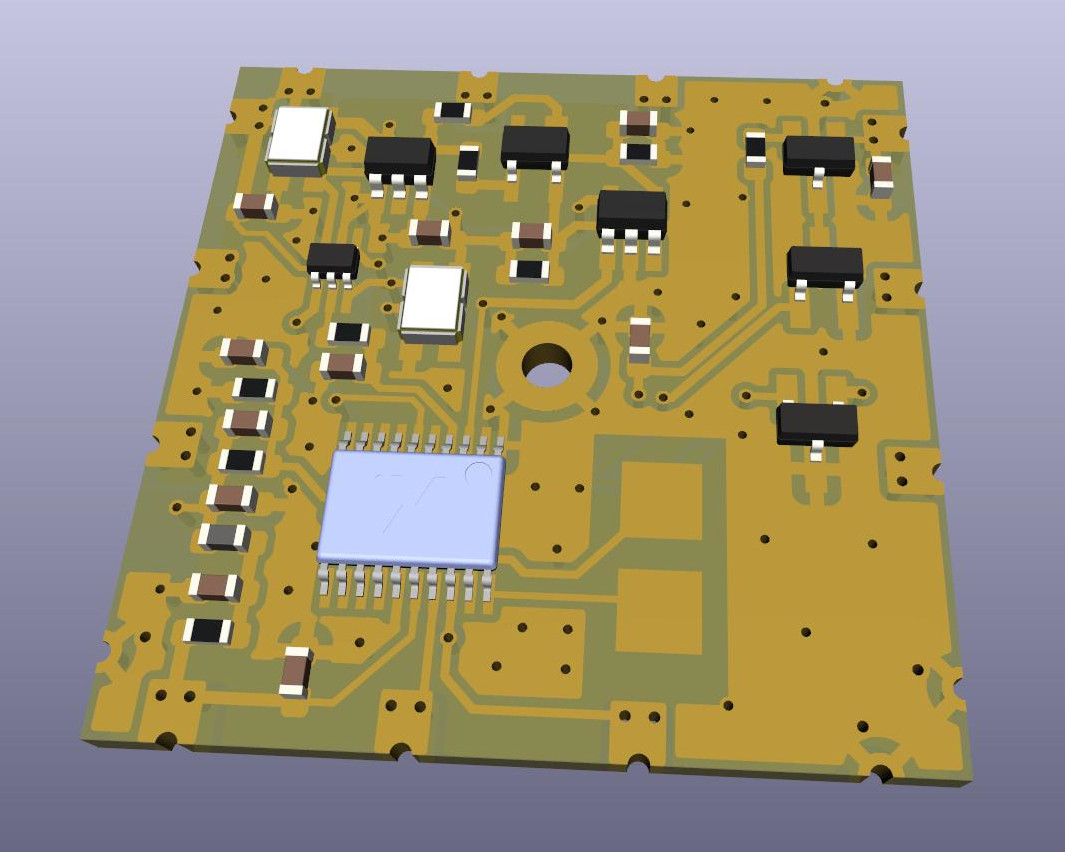
\includegraphics[width=0.5\textwidth]{3d_render}
	\caption{3D board image}
\end{figure}


% For wide tables, a single column layout is better. It can be switched
% page-by-page.
\onecolumn


\section{Electrical Specifications}
All specifications are in $-40\degree C \leq T_A \leq 85\degree C$ unless otherwise noted.

\begin{table}[h]
\begin{threeparttable}
	\caption{Electrical characteristic specifications}
\begin{tabularx}{\textwidth}{l | c | c c c | c | X}
    \thickhline
    \textbf{Parameter} & \textbf{Symbol} & \textbf{Min.} & \textbf{Typ.} & \textbf{Max.} &
    \textbf{Unit} \\
    \hline
    Current consumption  & $I_S$ & - & 10 & - & mA  \\
	Additional current consumption with spear oscillator On & $I_O$ & 6 & 7 & 8 & mA \\
	Additional current consumption with Hall sensor On & $I_H$ & - & 6 & 10 & mA \\
    \thickhline
\end{tabularx}
\begin{tablenotes}
\item[1]{Based on characterization data, not tested in production.}
\end{tablenotes}
\end{threeparttable}
\end{table}



\section{Dimensions}
All specifications are in $25\degree C$  unless otherwise noted.
\begin{table}[h]
\caption{Board Dimensions}
\begin{tabularx}{\textwidth}{l | X}
    \thickhline
    \textbf{Parameter} & \textbf{Size} \hspace{5cm} \\
    \hline
    Side & 30.0 x 30.0  \\
	Height & 3.0 \\
    \thickhline
\end{tabularx}
	\begin{tablenotes}
	\item[1]{Dimensions are expressed in millimeters.}
	\end{tablenotes}
\end{table}


\begin{table}[h]
\caption{Board weight (Guaranteed by design but not characteristic.)}
\begin{tabularx}{\textwidth}{l | X}
    \thickhline
	\textbf{Parameter} & \textbf{Max.}  \hspace{5cm} \\
    \hline
	Weight & 5 \\
	
    \thickhline
\end{tabularx}
	\begin{tablenotes}
	\item[1]{Units are expressed in gramm.}
	\end{tablenotes}
\end{table}

\newpage

\section{Commands}
\begin{table}[h]
\caption{User Commands}
\begin{tabularx}{\textwidth}{l | X}
    \thickhline
    \textbf{Parameter} & \textbf{Function} \hspace{5cm} \\
    \hline
   	R & Reboot \\
	Z & Zero state \\
	U & UART measurement\\
	N & ADC noise measurement\\
	H & Hall effect measurement\\
	Q & Quotes sending\\
	T & Temperature measurement\\
	E & No experiment\\
	V & Switch hall sensor VREF on\\
    \thickhline
\end{tabularx}
\end{table}




\begin{figure}
	\centering
	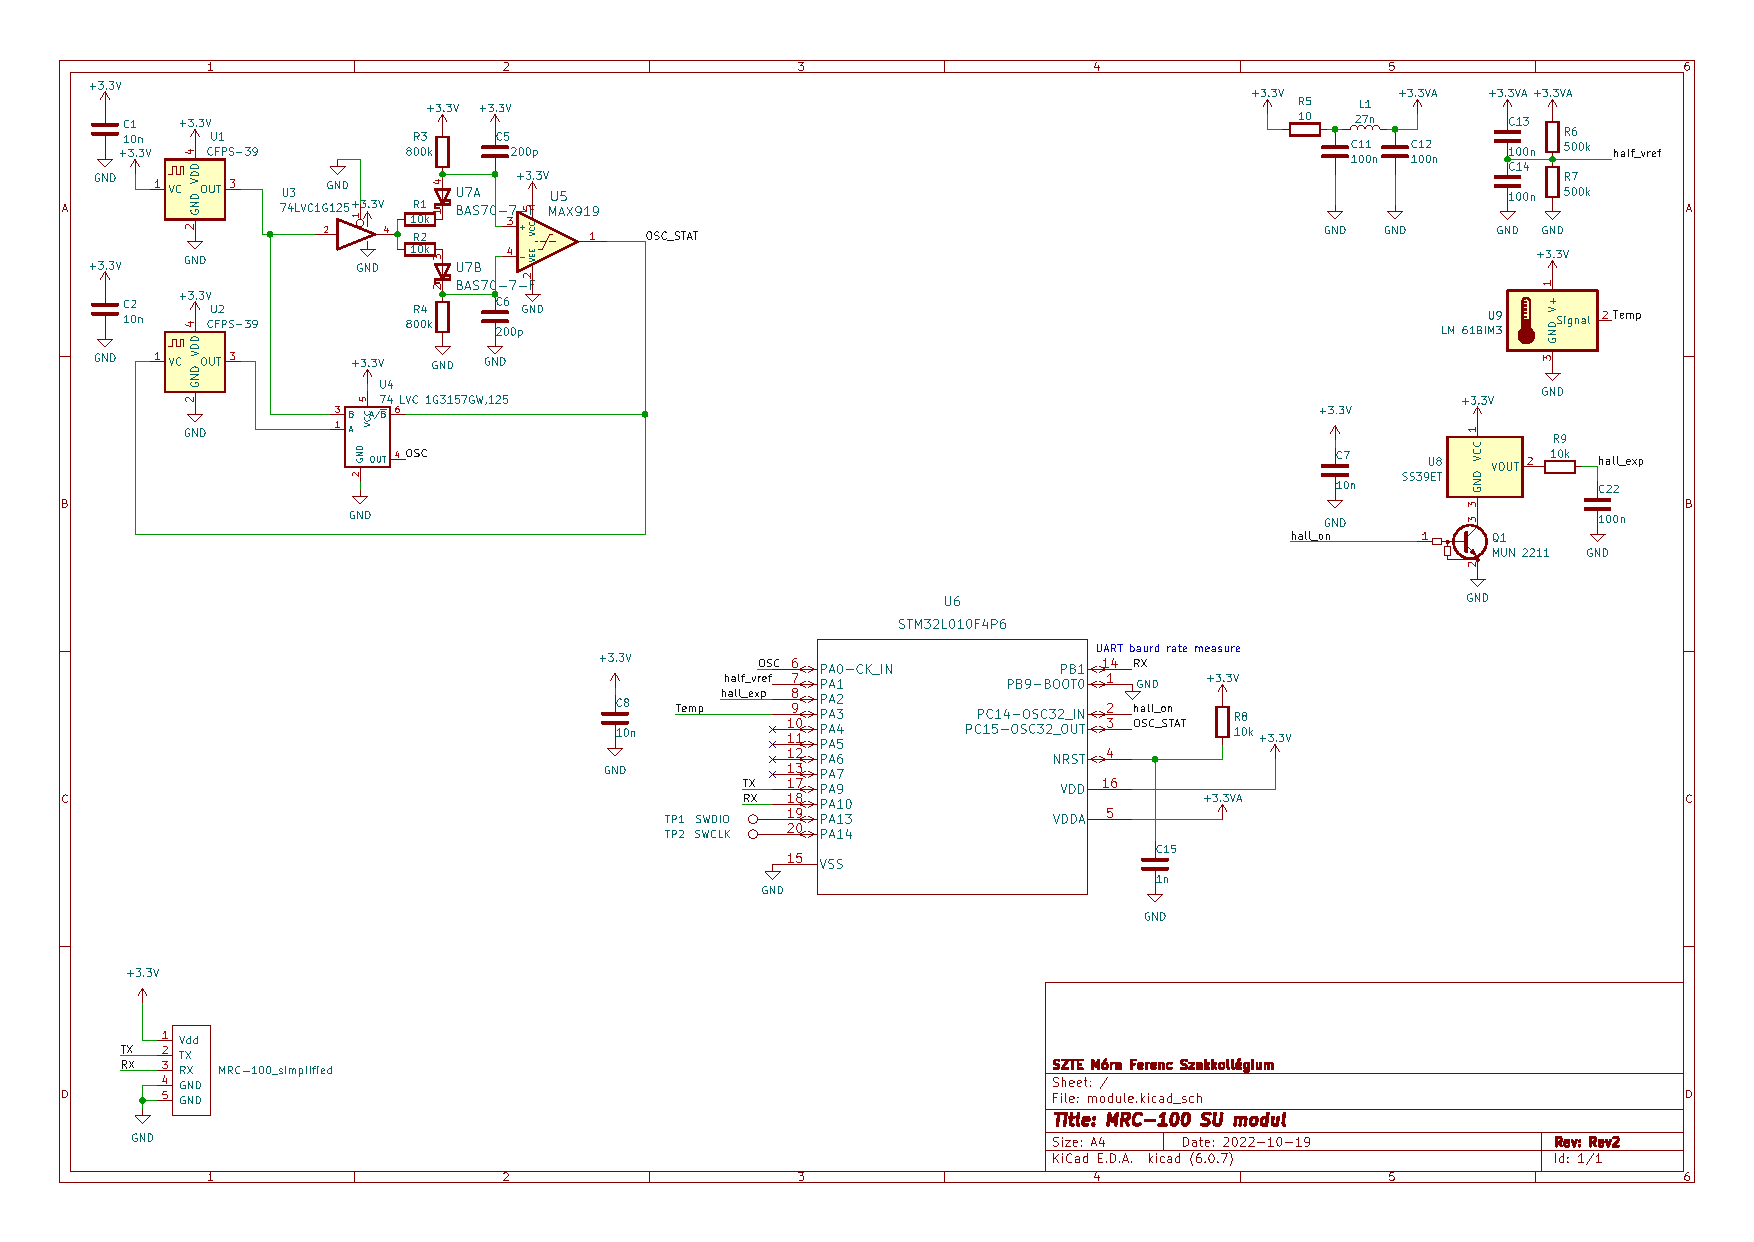
\includegraphics[width=1.2\textwidth,angle = 90]{sch}
	\caption{Schematics}
\end{figure}


\begin{figure}
	\centering
	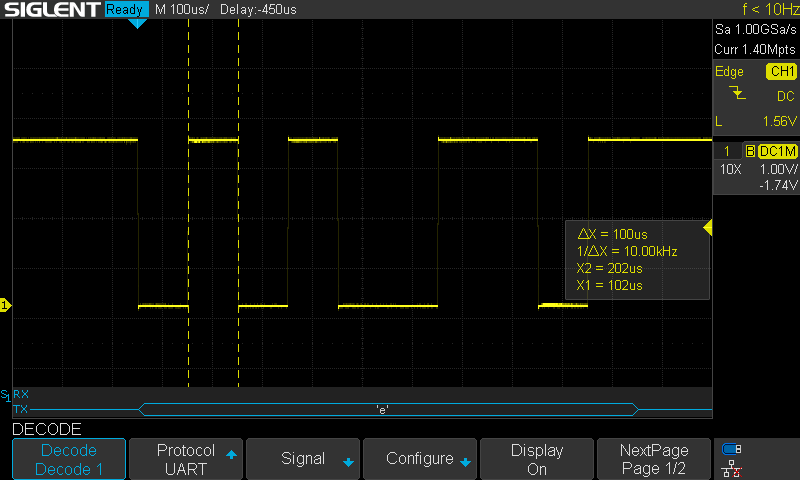
\includegraphics[width=1\textwidth]{SDS1}
	\caption{Universal Asynchronous Receiver-Transmitter frame waveform}
\end{figure}


\begin{figure}
	\centering
	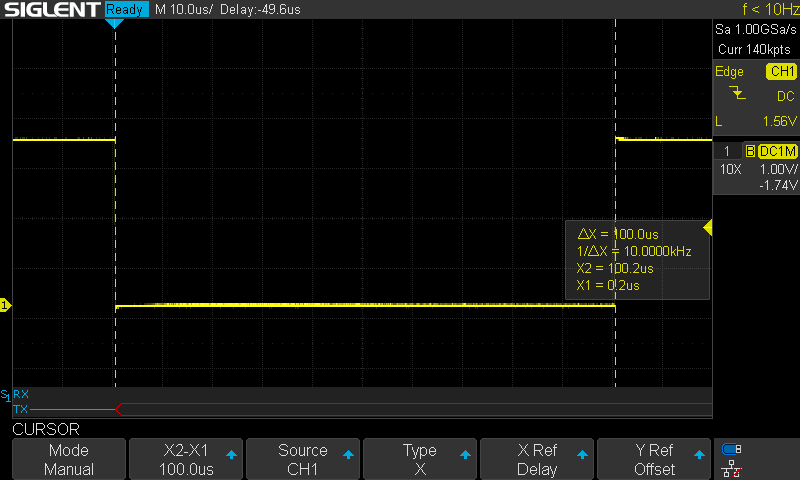
\includegraphics[width=1\textwidth]{SDS2}
	\caption{Universal Asynchronous Receiver-Transmitter bit time measure}
\end{figure}

\newpage
\section{Validation report}
\subsection{Mass}
\vspace{25mm}
\begin{tabular}{@{}C{1.5in}p{1in}C{1.5in}p{1in}C{1.5in}@{}}
	\hrulefill & \hfill & \hrulefill & \hfill & \hrulefill\\
	Instrument & \hfill & Mass & \hfill & Signature \\
\end{tabular}

\subsection{Current at $V_{in}=3.3V$}
\vspace{25mm}
\begin{tabular}{@{}C{1.5in}p{1in}C{1.5in}p{1in}C{1.5in}@{}}
	\hrulefill & \hfill & \hrulefill & \hfill & \hrulefill\\
	Instrument & \hfill & Current & \hfill & Signature \\
\end{tabular}

\subsection{Thermal-chamber}
\vspace{25mm}
\begin{tabular}{@{}C{1.5in}p{1in}C{1.5in}p{1in}C{1.5in}@{}}
	\hrulefill & \hfill & \hrulefill & \hfill & \hrulefill\\
	Instrument & \hfill & Pass & \hfill & Signature \\
\end{tabular}






\end{document}



